\chapter{Other works}


\section{Rajan Tranform and Set Theoretic Rajan Transform}

We planned to use the Set Theoretic Rajan Transform (STRT) in our process but it wasn't possible due to some issues and imprecisions in the documentation concerning the STRT$^{-1}$. We wanted to use this transformation on an image mainly because it has noise removal properties.

~~

The Set Theoretic Rajan Transform (STRT) correspond to the Rajan Transform (RT) applied on the sets domain. First I will present the forward rajan transform, and then it's application in the sets domain. Every equations, figures and explainations have been inspired by the following reference  \cite{bib:symbolic:RajanTransform}.

~~

The rajan transform take a sequence of $2^{i}$ numbers (the number of elements of the sequence have to be a power of 2), transform it, and return another sequence of $2^{i}$ numbers. We will call $x(k)$ the input sequence, $X(k)$ the output sequence of the tranform, and $N$ the number of element in the sequence \cite{bib:symbolic:RajanTransform}. 

~~

We can define the sequences $x(k)$, $g(k)$ and $h(k)$ as following : 
\begin{align}
x &= x(0), x(2), \cdots, x(k-1) & \text{where k is a power of 2} \\
g(k) &= x(k) + x(k + \frac{N}{2}) & \text{with } 0 \leq k \leq N / 2 \\
h(k) &= | x(k) - x(k - \frac{N}{2}) | & \text{with } N / 2 \leq k \leq N
\end{align}

~~

In other words, the sequence $x$ will be divided in two. Then we will sum the two first value of the subsequences (which will give us the results of $g(1)$), then the two seconds values (which is $g(2)$), then the thirds values, and so on until all the elements were processed. Then we will do the same operations but with a substraction instead (to get the sequence $h$).

~~

This processus will then have to be repeated on the subsequences $g$ and $h$ separately. We can see here the recursive character of this transformation. The figure \ref{fig:diagram:flowchart:rajan} illustrates the rajan tranformation in a more procedural way, with a sequence of 4 elements. 

\begin{figure}[H]
	\centering
	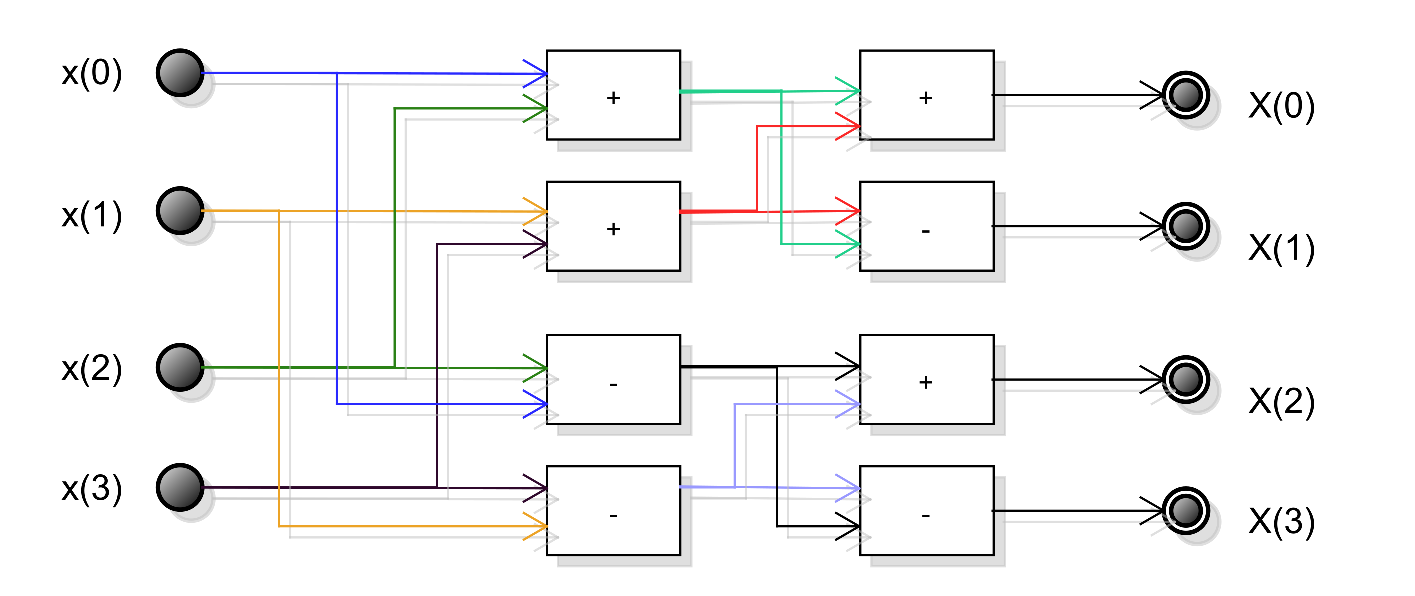
\includegraphics[width=0.7\textwidth]{images/diagrams/flowchart_rajan_transform}
	\caption{The forward Rajan Tranfform (RT)}
	\label{fig:diagram:flowchart:rajan}	
\end{figure}


The Set Theoretic Rajan Transform is the application of the Rajan Transform in the sets domain, and so instead of tranforming a sequence of numbers, it will tranform a sequence of sets, and return another sequence of sets (e.g. $x(1)$ and $X(1)$ wouldn't be numbers, but two sets). In the set domain, the addition correspond to the union, and the substraction to the difference of two sets.




